%!TEX root =../../../course-notes.tex
% ^ leave for LaTeXTools build functionality
\begin{applicationActivities}



\begin{activity}{10}
Determine which of the following ODEs are exact.
\begin{enumerate}[(a)]
\item \(\frac{dy}{dx}= \frac{-y}{x^2+y^2+x}\)
\item \( 1+\frac{x}{x^2+y^2} +\left(\frac{y}{x^2+y^2}\right)\frac{dy}{dx} = 0\)
\end{enumerate}
\end{activity}


\begin{activity}{15}
Solve the exact ODE 
\[ 1+\frac{x}{x^2+y^2} +\left(\frac{y}{x^2+y^2}\right)\frac{dy}{dx} = 0.\]
These solutions describe the trajectories taken by particles in the fluid flow below

\begin{center}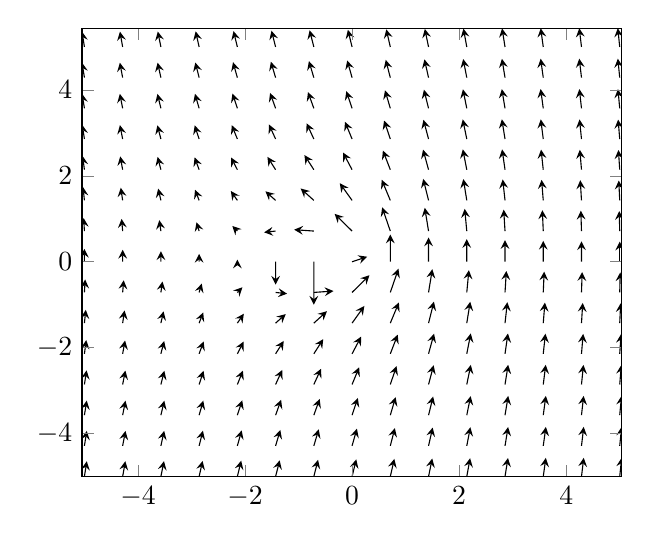
\begin{tikzpicture}
    \begin{axis}[
        domain=-5:5,
        view={0}{90},
        axis background/.style={fill=white},
    ]
        \addplot3[black,
            quiver={
             u={-y/(x^2+y^2)/(sqrt( (-y/(x^2+y^2))^2+(1+x/(x^2+y^2))^2)},
             v={1+x/(x^2+y^2)/(sqrt( (-y/(x^2+y^2))^2+(1+x/(x^2+y^2))^2)},
             scale arrows=0.4,
            },
            -stealth,samples=15]
                {exp(-x) - 1/2*sin(x) - 1/2*cos(x)};
    \end{axis}
\end{tikzpicture}\end{center}

\end{activity}



\begin{activity}{20}
Find solutions for the ODE
\[ 1+\frac{x}{x^2+y^2} +\left(\frac{y}{x^2+y^2}\right)\frac{dy}{dx} = 0\]
for each of the following initial conditions
\begin{enumerate}[(a)]
\item \(y(0)=-1\).
\item \(y(-2)=-2\).
\item \(y(-4)=-4\).
\end{enumerate}
Plot each of the solution curves.
\end{activity}




\end{applicationActivities}
